\section{Results}
\label{sec:results}

For evaluating our dataset generation, we first collected commits without any limits imposed on commits from
a single author. We later added a per-author limit in order to avoid bias being introduced by including a
vast amount of commits from a single author.

\autoref{fig:total_vs_tagged_with_limit} shows that around 25000 commits (~2.5\%) out of a total of 1000000
commits are tagged when limiting the number of commits per author to 100. Without this limit, the number of
tagged commits slightly increases to about 35000 commits (~3.5\%) out of 1000000, which is shown in
\autoref{fig:total_vs_tagged_without_limit}. Overall, we see that with or without limit, the number of tagged
commits remains relatively small compared to the total number of commits.

\begin{figure}[H]
  \centering
  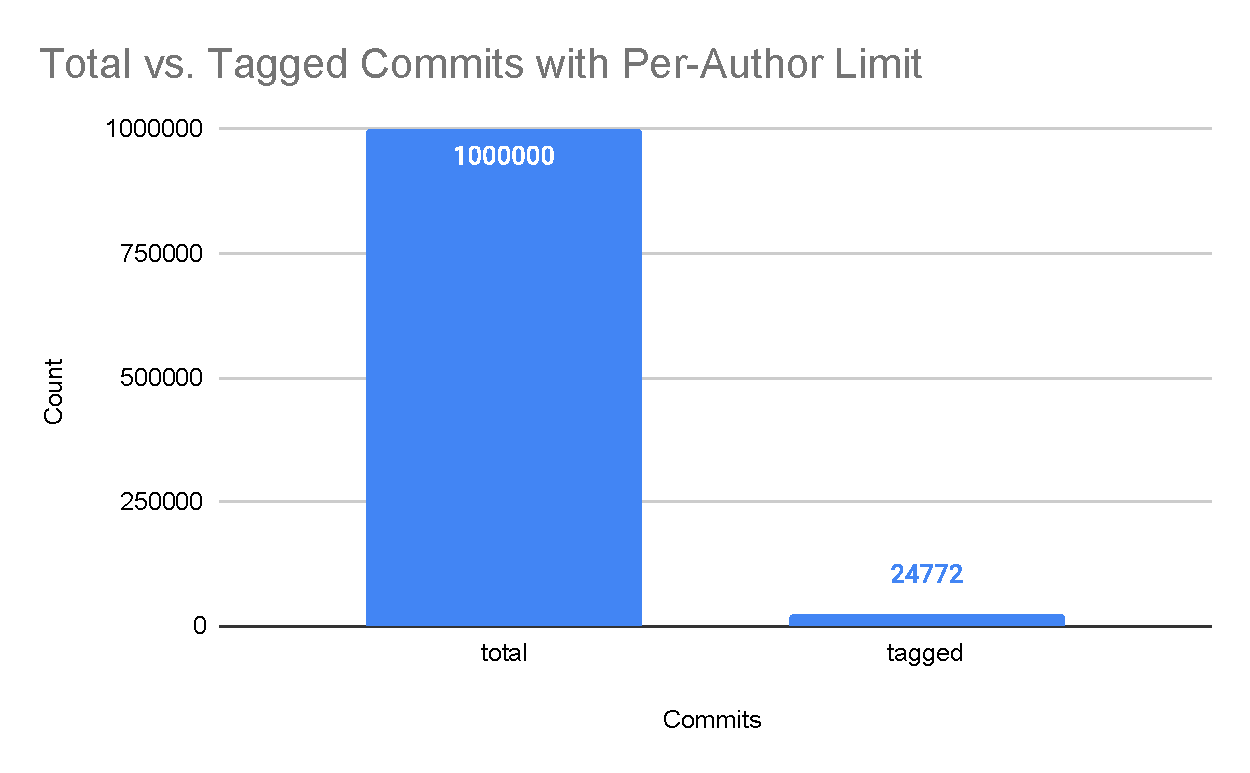
\includegraphics[width=\textwidth]{total-vs-tagged-commits-with-author-limit.pdf}
  \caption{Total vs. Tagged Commits with Per-Author Limit}
  \label{fig:total_vs_tagged_with_limit}
\end{figure}

\begin{figure}[H]
  \centering
  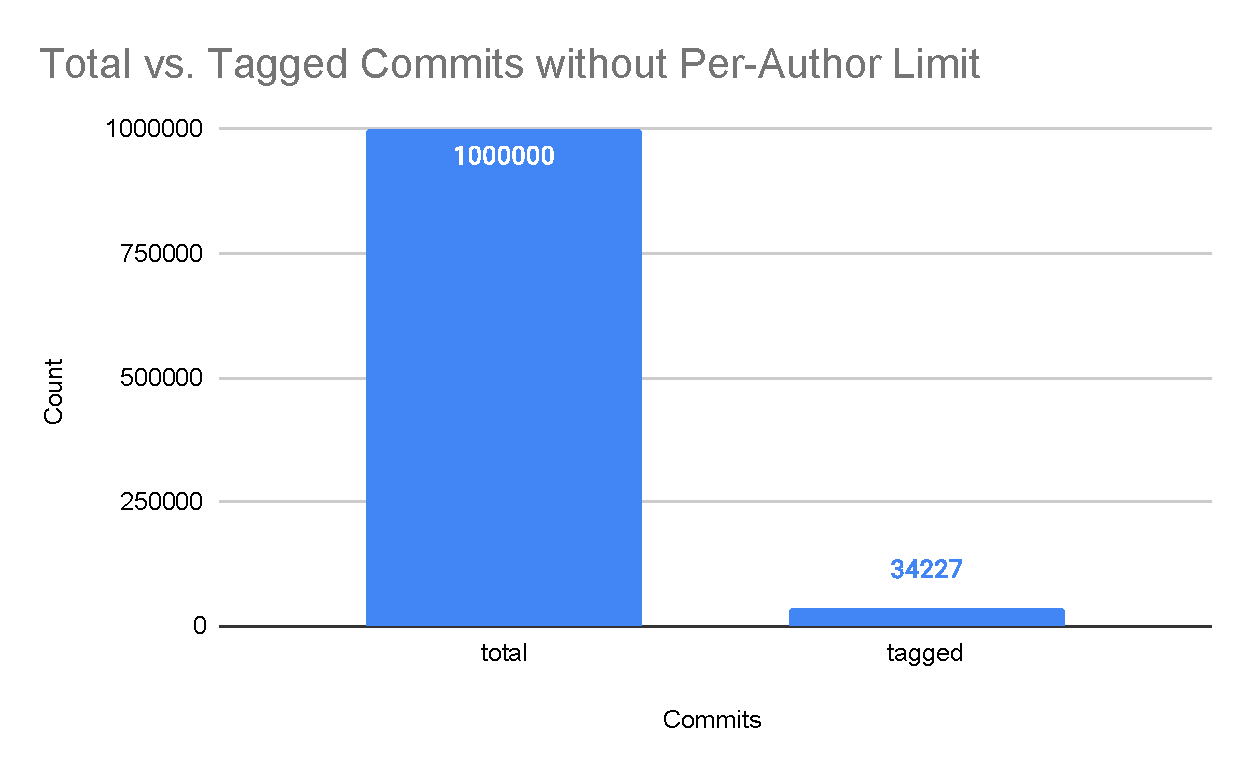
\includegraphics[width=\textwidth]{total-vs-tagged-commits-without-author-limit.pdf}
  \caption{Total vs. Tagged Commits without Per-Author Limit}
  \label{fig:total_vs_tagged_without_limit}
\end{figure}

In \autoref{fig:tag_dist_with_limit} and \autoref{fig:tag_dist_without_limit}, we can see the distribution
of commit tags with and without the mentioned per-author limit, respectively. When comparing both graphs,
we can see that without a per-author commit limit, the number of commits tagged with “chore” almost doubles
while commits tagged with “feat” stay more or less the same. This is likely due to commits being authored by
bots, which mainly applies to automatic maintenance tasks, i.e. chores.

\begin{figure}[H]
  \centering
  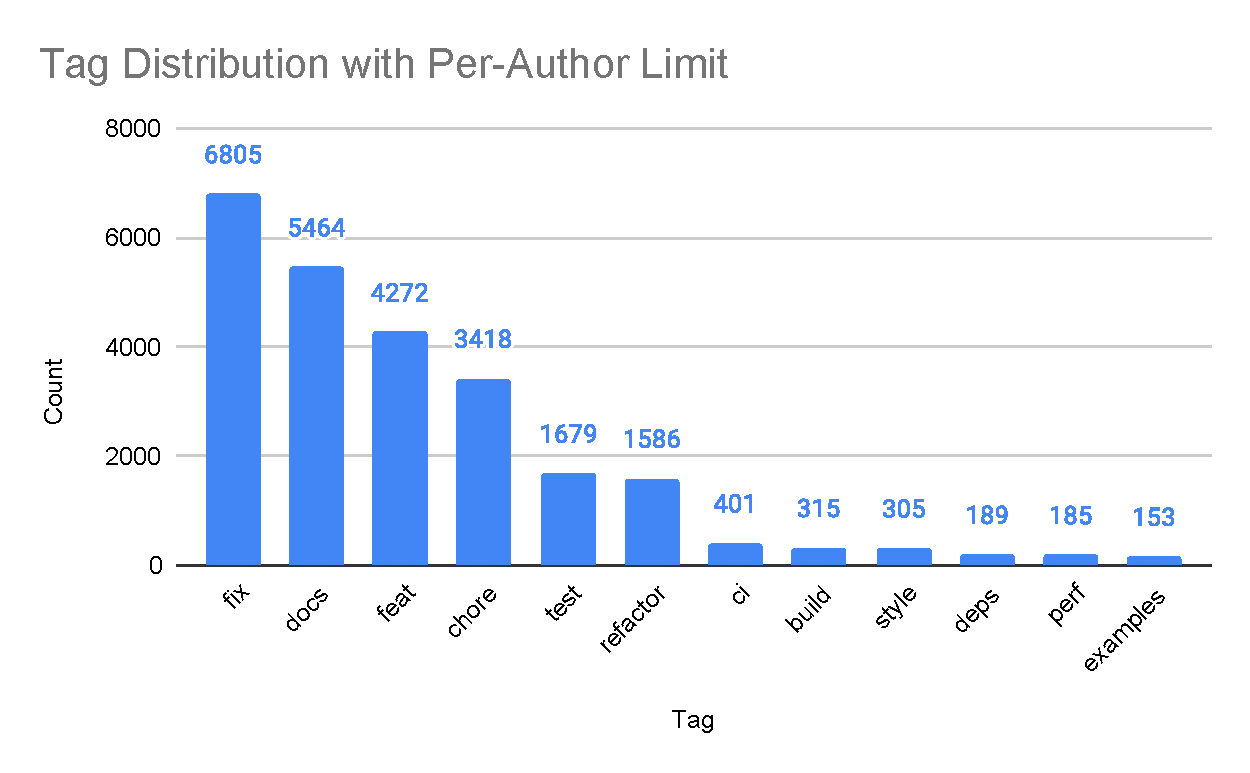
\includegraphics[width=\textwidth]{tag-distribution-with-author-limit.pdf}
  \caption{Tag Distribution with Per-Author Limit}
  \label{fig:tag_dist_with_limit}
\end{figure}

\begin{figure}[H]
  \centering
  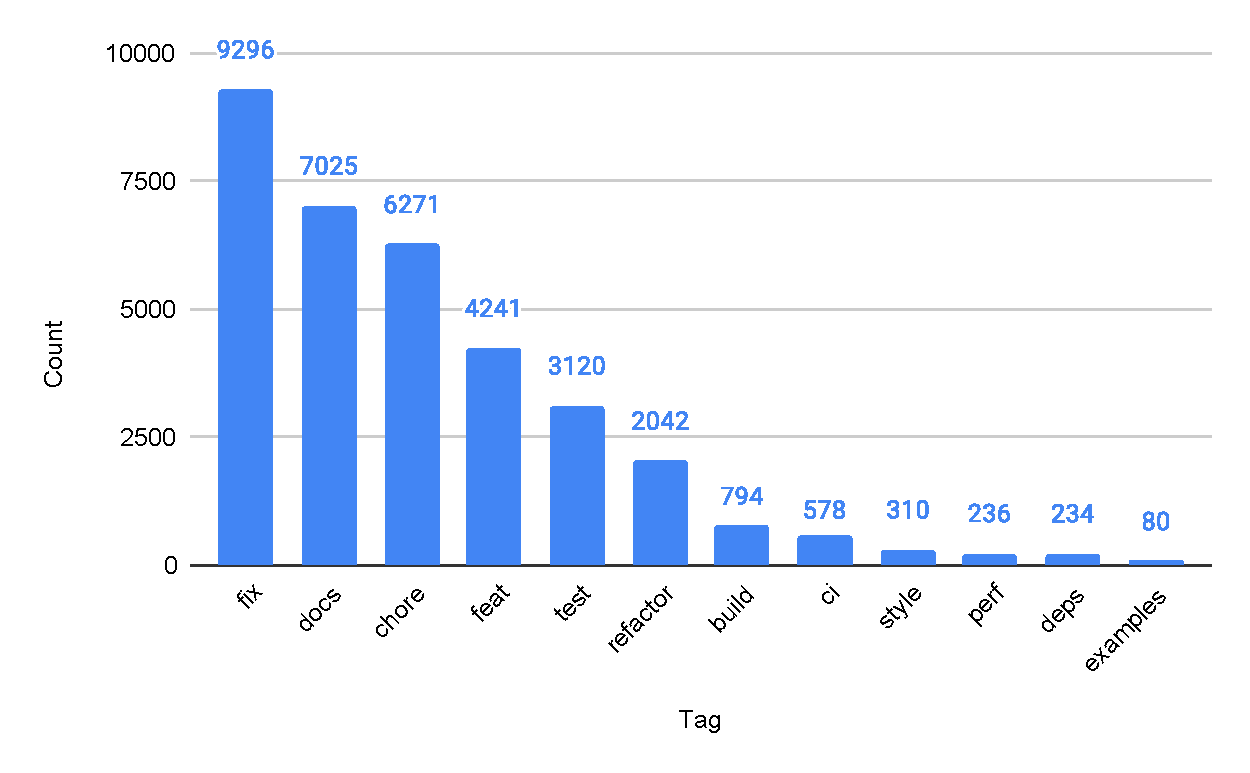
\includegraphics[width=\textwidth]{tag-distribution-without-author-limit.pdf}
  \caption{Tag Distribution without Per-Author Limit}
  \label{fig:tag_dist_without_limit}
\end{figure}

When comparing the results of the logistic regression, we can clearly notice a difference between the two sets.
With unlimited messages per author we get about ~4.15\% improvement over the set with author limitations. This
can be related to the bias introduced by authors contributing a very high amount of commit messages. We can
conclude from the distribution of labels that those authors primarily are maintenance bots, sticking to a
uniform commit message structure, which improves likelihood of correct classification.

Looking at the F1-score macro, we can further conclude that the high increase compared to the set with author
limits is due to those extra commits. As previously shown, the additional commits contain a high amount of
"chore" or "docs" tags, which directly relates them to bots. The uniformity of bot commits increases likelihood
of correct classification, resulting in high accuracy for those labels. As F1-macro does not consider the
proportion for each label in the dataset, we get a higher score for the set without author limitations.

The results however are very promising overall. When using the author limit, we are basically working with a
very balanced set in terms of commit message diversity while still getting acceptable results with an accuracy
of ~61.02\% and an F1-score micro of ~61.02\%. The lower F1-score macro of ~44.79\% is more likely to be a
result of insufficient training data, as half of the labels only have a small number of entries in the data set.
The exact results are displayed in \autoref{fig:unlimited_commits} and \autoref{fig:limited_commits}.

\begin{table}[H]
  \def\arraystretch{1.15}%
  \centering
  \begin{tabular}{|l|r|}
    \hline
    Accuracy       & 65.17\% \\
    \hline
    F1-score micro & 65.17\% \\
    \hline
    F1-score macro & 53.71\% \\
    \hline
  \end{tabular}
  \caption{Unlimited commit messages per author}
  \label{fig:unlimited_commits}
\end{table}

\begin{table}[H]
  \def\arraystretch{1.15}%
  \centering
  \begin{tabular}{|l|r|}
    \hline
    Accuracy       & 61.02\% \\
    \hline
    F1-score micro & 61.02\% \\
    \hline
    F1-score macro & 44.79\% \\
    \hline
  \end{tabular}
  \caption{100 commit messages per author}
  \label{fig:limited_commits}
\end{table}

